\documentclass{clbeamer2024}

\usepackage{minted}

\usepackage{minted}
\setminted{
	breaklines=true,
	frame=single,
	bgcolor=lightgray,
	fontsize=\small,
	escapeinside=||
}

\usepackage{xcolor}
\definecolor{bg}{rgb}{0.95, 0.95, 0.92} % Couleur gris clair

\title{
	%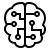
\includegraphics[width=0.5cm]{logos/IA1.png} \hfill
        Introduction à Scrum
	
\includegraphics[width=0.7cm]{logos/scrum.png} \hfill
}
\subtitle{Comprendre le cadre agile pour la gestion de projet}
\author{Slimani Mohamed Amine}
\institute{EHTP}
\date{\today}

\begin{document}
	\setcounter{framenumber}{-1}
	\frame{\titlepage}
	
	
	
	% Sommaire
	\begin{frame}{Sommaire}
		\tableofcontents
	\end{frame}
	
	
	\section{Qu'est-ce que Scrum ?}
	\begin{frame}{Qu'est-ce que Scrum ?}
		\begin{itemize}
			\item \textbf{Définition} : Scrum est un cadre agile pour la gestion de projet, principalement utilisé pour le développement de produits complexes.
			\item \textbf{Objectif} : Livrer des incréments de produit de manière itérative et incrémentale.
			\item \textbf{Avantages} : Flexibilité, transparence, et amélioration continue.
		\end{itemize}
	\end{frame}
	
	\section{Pourquoi utiliser Scrum ?}
	\begin{frame}{Pourquoi utiliser Scrum ?}
		\begin{itemize}
			\item \textbf{Flexibilité} : Permet de s'adapter rapidement aux changements.
			\item \textbf{Transparence} : Améliore la visibilité sur l'avancement du projet.
			\item \textbf{Collaboration} : Encourage la communication et la collaboration au sein de l'équipe.
		\end{itemize}
	\end{frame}
	
	\section{Les rôles dans Scrum}
	\begin{frame}{Les rôles dans Scrum}
		\begin{itemize}
			\item \textbf{Product Owner} : Responsable de maximiser la valeur du produit et de gérer le Product Backlog.
			\item \textbf{Scrum Master} : Facilite le processus Scrum et aide l'équipe à suivre les pratiques Scrum.
			\item \textbf{Équipe de développement} : Responsable de la livraison des incréments de produit à la fin de chaque Sprint.
		\end{itemize}
	\end{frame}
	
	\section{Les événements Scrum}
	\begin{frame}{Les événements Scrum}
		\begin{itemize}
			\item \textbf{Sprint} : Période de temps fixe (généralement 2-4 semaines) pendant laquelle un incrément de produit est livré.
			\item \textbf{Sprint Planning} : Réunion pour planifier les tâches du Sprint.
			\item \textbf{Daily Scrum} : Réunion quotidienne de 15 minutes pour synchroniser l'équipe.
			\item \textbf{Sprint Review} : Réunion pour présenter l'incrément de produit aux parties prenantes.
			\item \textbf{Sprint Retrospective} : Réunion pour améliorer le processus Scrum.
		\end{itemize}
	\end{frame}
	
	\section{Les artéfacts Scrum}
	\begin{frame}{Les artéfacts Scrum}
		\begin{itemize}
			\item \textbf{Product Backlog} : Liste priorisée des fonctionnalités et tâches à réaliser.
			\item \textbf{Sprint Backlog} : Liste des tâches sélectionnées pour le Sprint en cours.
			\item \textbf{Incrément} : Résultat tangible du Sprint, prêt à être livré.
		\end{itemize}
	\end{frame}
	
	\section{Exemple de Sprint Planning}
	\begin{frame}[fragile]{Exemple de Sprint Planning}
		\begin{exampleblock}{Étapes du Sprint Planning}
			\begin{enumerate}
			
				\item Le Product Owner présente les éléments prioritaires du Product Backlog.
				\item L'équipe de développement discute des tâches et estime l'effort nécessaire.
				\item L'équipe sélectionne les tâches pour le Sprint.
				\item Définition des objectifs du Sprint.
			\end{enumerate}
		\end{exampleblock}
	\end{frame}
	
	
	\section{Exemple de Daily Scrum}
	\begin{frame}[fragile]{Exemple de Daily Scrum}
		\begin{exampleblock}{Questions typiques du Daily Scrum}
			\begin{enumerate}
				\item Qu'avez-vous fait hier ?
				\item Que ferez-vous aujourd'hui ?
				\item Y a-t-il des obstacles qui vous empêchent de progresser ?
			\end{enumerate}
		\end{exampleblock}
	\end{frame}
	
	
	\section{Bonnes pratiques}
	\begin{frame}{Bonnes pratiques}
		\begin{itemize}
			\item \textbf{Respect des rôles} : Chaque membre de l'équipe doit comprendre et respecter son rôle.
			\item \textbf{Transparence} : Toutes les informations doivent être visibles et accessibles à l'équipe.
			\item \textbf{Amélioration continue} : Utiliser la rétrospective pour identifier et implémenter des améliorations.
		\end{itemize}
	\end{frame}
	
	
	\section{Outils pour Scrum}
	\begin{frame}{Outils pour Scrum}
		\begin{itemize}
			\item \textbf{Jira} : Outil populaire pour gérer les backlogs et suivre les Sprints.
			\item \textbf{Trello} : Tableau visuel pour gérer les tâches et les Sprints.
			\item \textbf{Confluence} : Outil de documentation pour les Product Backlogs et les réunions.
		\end{itemize}
	\end{frame}
	
	\section{Défis de Scrum}
	\begin{frame}{Défis de Scrum}
		\begin{itemize}
			\item \textbf{Engagement} : Nécessite un engagement fort de toute l'équipe.
			\item \textbf{Changement de culture} : Peut nécessiter un changement de culture organisationnelle.
			\item \textbf{Gestion des priorités} : Le Product Owner doit constamment prioriser les tâches.
		\end{itemize}
	\end{frame}	
	
	
	\section{Pourquoi c'est important ?}
	\begin{frame}{Pourquoi c'est important ?}
		\begin{itemize}
			\item Scrum permet de livrer des produits de haute qualité de manière itérative et incrémentale.
			\item Il améliore la collaboration et la communication au sein des équipes.
			\item Comprendre Scrum est essentiel pour les équipes de développement et les chefs de projet.
		\end{itemize}
	\end{frame}
	
	
	\begin{frame}{Résumé}
		\textbf{Scrum} est un cadre agile puissant pour la gestion de projet, permettant de livrer des produits de manière itérative et incrémentale.  
		Explorez, apprenez, et appliquez Scrum dans vos projets !
	\end{frame}
	
	
	

	

	
\end{document}
